\documentclass[main.tex]{subfile}

\begin{document}

\section{Second Order Differential Equations}
\label{sec:seAnalaysis}

\subsection{Background}
\label{sec:background}

A second order ODE can be seen by chaining two Butterworth filters together as
shown in \figref{seCircuit}.

\begin{figure}[H]
	\begin{center}
		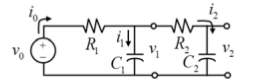
\includegraphics{seCircuit}
	\end{center}
	\caption{Second Order Butterworth filter (graphic taken from lab manual)}
	\label{fig:seCircuit}
\end{figure}

To find the output voltage of the filter we use the following equations to
derive the differential equation:

\begin{align*}
	V_0 &= i_0R_1 + V_1
	\\V_1 &= i_2R_2 + V_2
	\\i_0 &= i_1 + i_2
	\\i_j &= \frac{dV_j}{dt}C_j
\end{align*}

By substitution we arive at our second order ODE:

\begin{align}
	V_0 &= \frac{d^2V_2}{dt^2}(C_1C_2R_1R_2) + \frac{dV_2}{dt}(C_2R_1 + R_2) + V_2(C_1R_1 + 1)
	\\V_0 &= \frac{d^2V_2}{dt^2}(\alpha) + \frac{dV_2}{dt}(\beta) + V_2(\gamma)
\end{align}

For this lab we assume that $\alpha$, $\beta$, and $\gamma$ are set such that
the system is underdamped with the natural frequency being $\omega_n = 15\pi$
and the damping ration as $\xi = \frac{1}{\sqrt{2}}$. From equation $2.20$ in
the textbook $\alpha$, $\beta$, and $\gamma$ coorespond to $m$, $c$, and $k$
which are the constants of a mass-spring-damper mechanical system. For any
second order system the theoretical the percent-overshoot is described by
\eqref{pos}.

\begin{align}
	\%OS = 100 e^{-\xi \frac{\pi}{\sqrt{1-\xi^2}}} \label{eq:pos}
\end{align}

For our expirements therefore $\%OS \approx 4.3214 \%$

\subsection{Expiremental Determination of \%OS}
\label{sec:expiremental_determination_of_}

As with the first order system we use \Labview to simulate a second order
Butterworth filter. We perform the following steps to create the filter: 

\begin{enumerate}
	\item Create a signal generation block to output a square wave with a
		frequency of $1\dem{Hz}$. This simulates a step input to our filter at
		a frequency low enough to drive the system well beyond its settling time.
	\item Next we create a filter block diagram (found in the Express-Signal
		Analysis section of the toolbox) to create a Butterworth filter. We set the
		filter to be a second-order system with natural frequency and damping ratio
		as described above.
	\item Finally we add graphs to the outputs of both signal generator and filter
		block diagrams.
\end{enumerate}

\begin{figure}[H]
	\begin{center}
		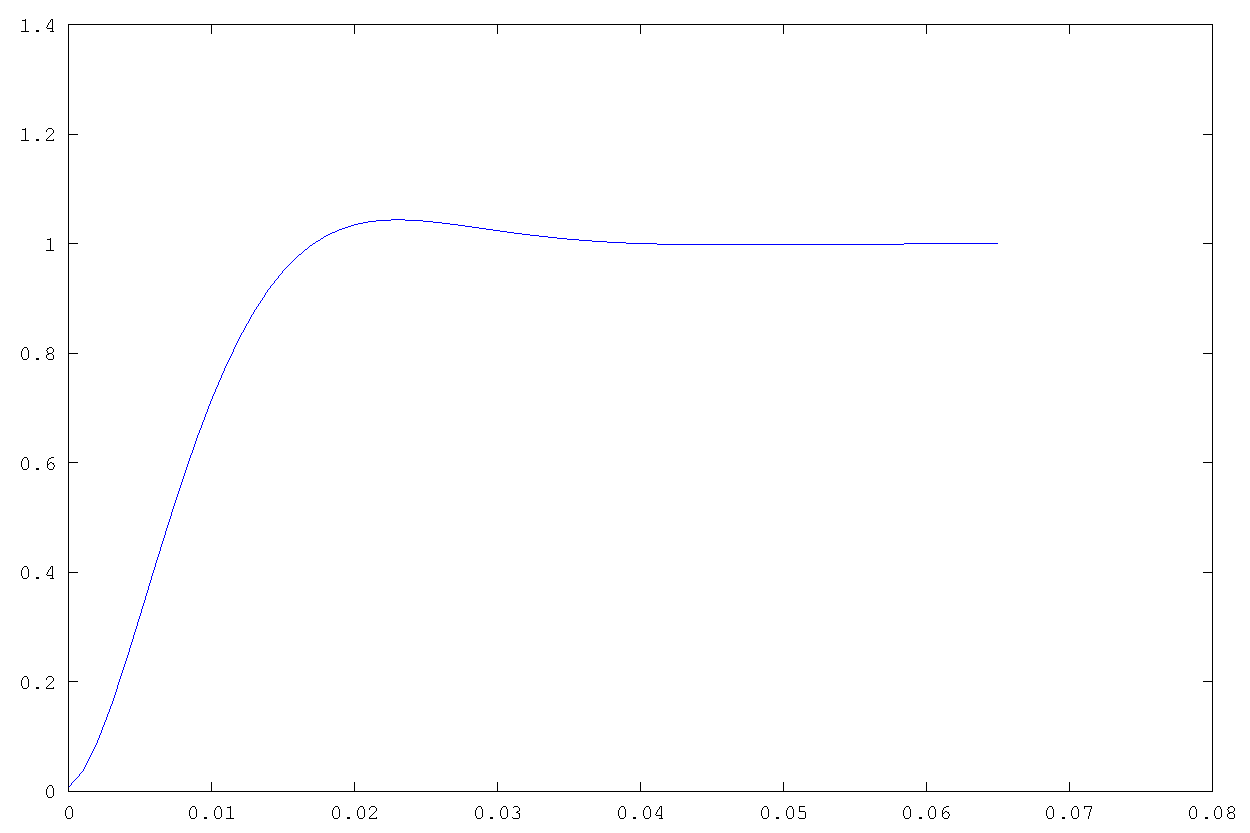
\includegraphics[width=\linewidth]{seAnalResponse.pdf}
	\end{center}
	\caption{Second Order Butterworth Response}
	\label{fig:seGraph}
\end{figure}

\figref{seGraph} shows the system response of the second order Butterworth
filter. Expirmentally the percent-overshoot is determined by \eqref{exPos}:

\begin{align}
	\%OS_{\text{exp}} = \frac{y_{\text{max}} - y_{\text{ss}}}{y_{\text{ss}}}
	\label{eq:exPos}
\end{align}
where $y_{\text{max}}$ is the maximum value of the system output and
$y_{\text{ss}}$ is the steady state value of the system. In our case
$y_{\text{max}} \approx 1.0438$ and $y_{\text{ss}} = 1$.

For our system we calculated $\%OS_{\text{exp}} \approx 4.383$ which, relative
to our theoretical value, has a percent error of $\%1.4257$. With such a small
error we deem that the simulation and theoretical values for percent-overshoot
agree. From this we can say that Labview accurately simulates realworld systems
that can be modeled by differential equations.

% subsection expiremental_determination_of_%os (end)

% subsection background (end)

% section seAnalaysis (end)

\end{document}
